%%%%%%%%%%%%%%%%%%%%%%%%%%%%%%%%%%%%%%%%%
% Beamer Presentation
% LaTeX Template
% Version 1.0 (10/11/12)
%
% This template has been downloaded from:
% http://www.LaTeXTemplates.com
%
% License:
% CC BY-NC-SA 3.0 (http://creativecommons.org/licenses/by-nc-sa/3.0/)
%
%%%%%%%%%%%%%%%%%%%%%%%%%%%%%%%%%%%%%%%%%

%----------------------------------------------------------------------------------------
%	PACKAGES AND THEMES
%----------------------------------------------------------------------------------------

\documentclass{beamer}

\mode<presentation> {

% The Beamer class comes with a number of default slide themes
% which change the colors and layouts of slides. Below this is a list
% of all the themes, uncomment each in turn to see what they look like.

%\usetheme{default}
%\usetheme{AnnArbor}
%\usetheme{Antibes}
%\usetheme{Bergen}
%\usetheme{Berkeley}
%\usetheme{Berlin}
%\usetheme{Boadilla}
%\usetheme{CambridgeUS}
%\usetheme{Copenhagen}
%\usetheme{Darmstadt}
%\usetheme{Dresden}
%\usetheme{Frankfurt}
%\usetheme{Goettingen}
%\usetheme{Hannover}
%\usetheme{Ilmenau}
%\usetheme{JuanLesPins}
%\usetheme{Luebeck}
\usetheme{Madrid}
%\usetheme{Malmoe}
%\usetheme{Marburg}
%\usetheme{Montpellier}
%\usetheme{PaloAlto}
%\usetheme{Pittsburgh}
%\usetheme{Rochester}
%\usetheme{Singapore}
%\usetheme{Szeged}
%\usetheme{Warsaw}

% As well as themes, the Beamer class has a number of color themes
% for any slide theme. Uncomment each of these in turn to see how it
% changes the colors of your current slide theme.

%\usecolortheme{albatross}
%\usecolortheme{beaver}
%\usecolortheme{beetle}
%\usecolortheme{crane}
\usecolortheme{dolphin}
%\usecolortheme{dove}
%\usecolortheme{fly}
%\usecolortheme{lily}
%\usecolortheme{orchid}
%\usecolortheme{rose}
%\usecolortheme{seagull}
%\usecolortheme{seahorse}
%\usecolortheme{whale}
%\usecolortheme{wolverine}

%\setbeamertemplate{footline} % To remove the footer line in all slides uncomment this line
\setbeamertemplate{footline}[page number] % To replace the footer line in all slides with a simple slide count uncomment this line

%\setbeamertemplate{navigation symbols}{} % To remove the navigation symbols from the bottom of all slides uncomment this line
}

\usepackage{graphicx} % Allows including images
\usepackage{booktabs} % Allows the use of \toprule, \midrule and \bottomrule in tables
\usepackage[absolute,overlay]{textpos}
\usepackage{multicol}

%\hypersetup{
%	colorlinks = true,
%	linkcolor = red
%}

%\makeatletter
%\let\@mycite\@cite
%\def\@cite#1#2{{\hypersetup{linkcolor=green!60!black}[{#1\if@tempswa , #2\fi}]}}
%\makeatother



%----------------------------------------------------------------------------------------
%	TITLE PAGE
%----------------------------------------------------------------------------------------

\title[Interring programs structure from an execution trace]
{
	\textit{Master thesis} \\
	Master in Research and Innovation \\
	\vspace{0.5cm}
	%\hrulefill \\
	\textbf{Inferring programs structure from \\
		an execution trace} \\
	%\hrulefill \\
}

\author
{
	Juan Francisco Mart\'inez Vera
}
\institute[FIB, UPC]
{
	Facultat d'Inform\`atica de Barcelona (FIB) \\
	Universitat Polit\`ecnica de Catalunya (UPC)
	\begin{figure}
		
\includegraphics[width=30px]{imgs/logo_upc.png}
	\end{figure}
}
\date{\today}

\AtBeginSection[]
{
	\begin{frame}<beamer>
		\frametitle{Outline for section \thesection}
		\tableofcontents[currentsection]
	\end{frame}
}

\begin{document}
%\logo{
\includegraphics[height=0.5cm]{imgs/logo_upc.png}}

\begin{frame}
\titlepage
\end{frame}

\begin{frame}[allowframebreaks]
\frametitle{Presentation outline}
\tableofcontents
\end{frame}

%----------------------------------------------------------------------------------------
%	PRESENTATION SLIDES
%----------------------------------------------------------------------------------------

\section{Context}
\subsection{High Performance Computing}
\begin{frame}
\frametitle{High Performance Computing}
\begin{itemize}
	\item Becomes the third support of science with mathematics and theory
	\item Tremendous improvement in all transformation hierarchy layers
\end{itemize}
\pause
\begin{figure}
	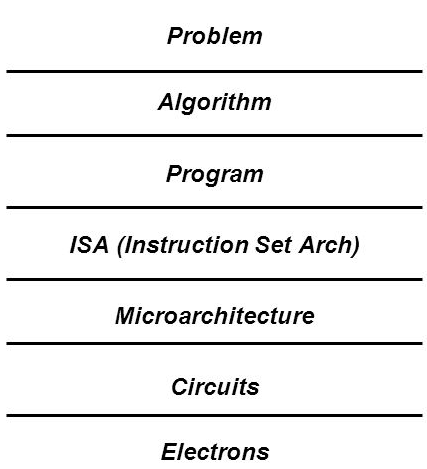
\includegraphics[width=100px]{imgs/transformationhierarchy.png}
	\caption{Transformation hierarchy}
\end{figure}
\begin{textblock*}{5cm}(40px,160px) % {block width} (coords)
	\includegraphics<+(1)->[width=70px]{imgs/moore_prediction.png}
\end{textblock*}
\begin{textblock*}{5cm}(40px,100px) % {block width} (coords)
	\includegraphics<+(1)->[width=70px]{imgs/microarchitecture.png}
\end{textblock*}
\begin{textblock*}{5cm}(270px,170px) % {block width} (coords)
	\includegraphics<+(1)->[width=70px]{imgs/multicore.png}
\end{textblock*}
\begin{textblock*}{5cm}(270px,100px) % {block width} (coords)
	\includegraphics<+(1)->[width=70px]{imgs/program_simulation.png}
\end{textblock*}
\end{frame}

\subsection{Performance Analysis tools}
\begin{frame}
\frametitle{Performance Analysis tools (i)}
\begin{itemize}
	\item Focused on Program layer
	\item Aid to detect bottlenecks
	\item Is a cyclic process
	\begin{itemize}
		\item Less iterations better
		\item Depens on quality of hypothesis
		\item That is strongly related with possibilities tools provides
	\end{itemize}
\end{itemize}
\begin{figure}
	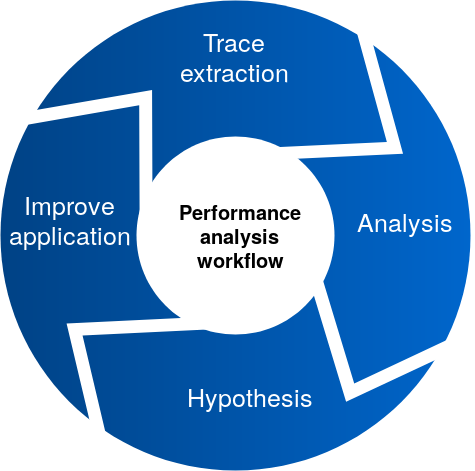
\includegraphics[width=100px]{imgs/performance_analysis_diagram.png}
	\caption{Performance analysis workflow}
\end{figure}
\end{frame}

\begin{frame}
\frametitle{Performance Analysis tools (ii)}
\begin{itemize}
	\item Have been demonstrate to be valuable on detection of bottlenecks
	\item Demands high skilled analysts
	\item So developers use to delegate this work
	\begin{itemize}
		\item \textbf{Analyst have to work with codes they are not familiar with}
	\end{itemize}
\end{itemize}
\begin{figure}
	
\includegraphics[width=100px]{imgs/pop.png}
	\caption{Performance optimisation and Productivity project}
\end{figure}
\pause
\begin{block}{Motivation 1}
	Providing application structure will lead to better understandability about what the application is doing.
\end{block}
\end{frame}

\begin{frame}
\frametitle{Performance Analysis tools (iii)}
\begin{itemize}
	\item When dealing with big traces:
	\begin{itemize}
		\item Visualizers responsiveness times \textbf{becomes prohibitive}
	\end{itemize}
	\item Analysis phases is then break down into:
	\begin{enumerate}
		\item Filter
		\item Cutter
		\item Inspection
	\end{enumerate}
\end{itemize}
\begin{figure}
	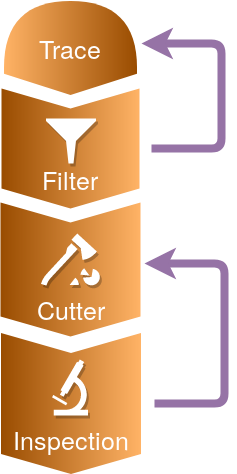
\includegraphics[width=40px]{imgs/analysis_subphases.png}
%	\caption{Analysis subphases}
\end{figure}
\pause
\begin{block}{Motivation 2}
	Having the structure of the application will aid the process of identify regions of interest
\end{block}
\end{frame}

\section{State of the Art}
\subsection{Syntactic structure}

\begin{frame}
\frametitle{State of the Art (i)}
\begin{itemize}
	\item On-line analysis
	\begin{itemize}
		\item In \cite{noeth2009scalatrace} propose structure derection for on-line trace compression
		\begin{itemize}
			\item Rely on \textbf{detecting and aggregating patterns}
		\end{itemize}
		\item In \cite{aguilar2016event} propose structure detection for on-line trace compression and visual performance analysis
		\begin{itemize}
			\item Rely on \textbf{directed graph construction} and DFS-analysis for cycles hierarchical analysis.
		\end{itemize}
	\end{itemize}
	\item Off-line analysis
	\begin{itemize}
		\item In \cite{Safyallah2006} propose improving reverse engineering by structure detection analysis
		\begin{itemize}
			\item Rely on \textbf{sequential pattern mining} techniques.
		\end{itemize}
		\item In \cite{Lopez-Cueva2012} propose to aid huge SoC traces
		\begin{itemize}
			\item Rely on \textbf{frequent periodic pattern mining}.
		\end{itemize}
		\item In \cite{trahay2015selecting} propose to select automatically the performance hotspots
		\begin{itemize}
			\item Rely on \textbf{growing sequential pattern mining}.
		\end{itemize}
	\end{itemize}
\end{itemize}
\end{frame}

\begin{frame}
\frametitle{State of the Art (ii)}
\begin{itemize}
	\item On-line analysis
	\begin{itemize}
		\item \cite{noeth2009scalatrace} By avoiding $O(n^{2})$ they \textbf{limits pattern recognition}
		\item In \cite{aguilar2016event} \textbf{Loss temporality} when detecting hierarchical structure
	\end{itemize}
	\item Off-line analysis
	\begin{itemize}
		\item \cite{Safyallah2006} \cite{Lopez-Cueva2012} \cite{trahay2015selecting} relies on pattern mining techniques that presents \textbf{high complexity}.
	\end{itemize}
\end{itemize}
\pause
\begin{block}{Motivation 3}
	Been scalable by finding out an alternative technique
\end{block}
\end{frame}

\section{Proposal}
\subsection{Application structure by classification}
\begin{frame}
\frametitle{Application structure by classification(i)}
HPC applications idiosincracy
\begin{itemize}
	\item Big outer loop
	\item Repetitive and stable executions
	\item Communications lies on loops that drives the execution
\end{itemize}
\vfill
\begin{multicols*}{3}
	\begin{figure}
		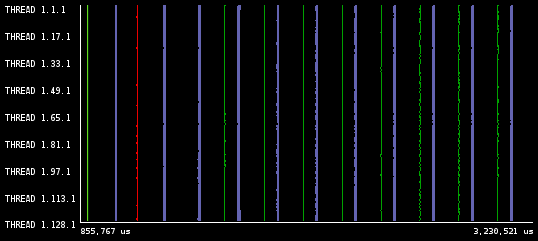
\includegraphics[width=0.3\textwidth,height=60px]{imgs/ft_trace_128.png}
		\caption{FT 128 ranks}
	\end{figure}
	
	\begin{figure}
		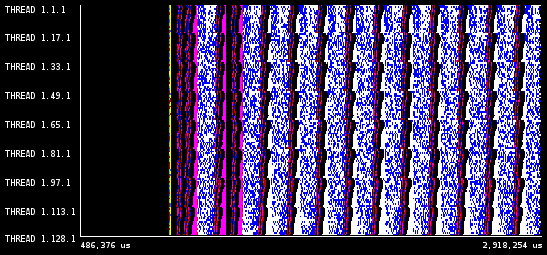
\includegraphics[width=0.3\textwidth,height=60px]{imgs/lu_trace_128.png}
		\caption{LU 128 ranks}
	\end{figure}
	
	\begin{figure}
		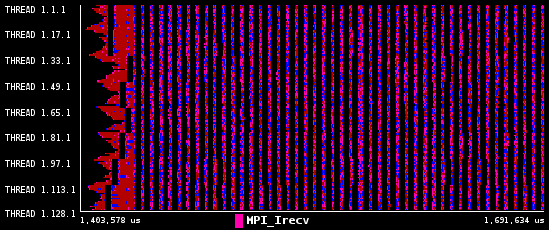
\includegraphics[width=0.3\textwidth,height=60px]{imgs/cg_trace_128.png}
		\caption{CG 128 ranks}
	\end{figure}

\end{multicols*}
\end{frame}

\begin{frame}
\frametitle{Application structure by classification (ii)}
\begin{itemize}
	\item Instead of following the trend, different proposal
	\item Taking into account the characteristics of our target
	\item Loops can be discovered by monitoring the communications
	\item Stable executions implies same behaviour for all iterations in a given loop
	\item So...
\end{itemize}
\vfill
\pause
\begin{block}{The key idea}
	Communications are used as proxies for the observation of iterations. Clustering them by its behaviour the applications structures can be betrayed.
\end{block}
\end{frame}

\begin{frame}
\frametitle{Application structure by classification (iii)}
Selected features must be able to
\begin{itemize}
	\item Join MPIs from the same loop
	\item Separe MPIs from different loops
\end{itemize}
\vfill
\pause
As a starting point ...
\begin{enumerate}
	\item \textbf{Number of repetitions}: Two different mpi calls in same loop will be executed the same ammount of time
	\item \textbf{Mean time between repetitions}: Two different loops will, presumibly, execute different work
\end{enumerate}
\end{frame}

\subsection{Workflow}
\begin{frame}
\frametitle{Workflow}
\begin{figure}
	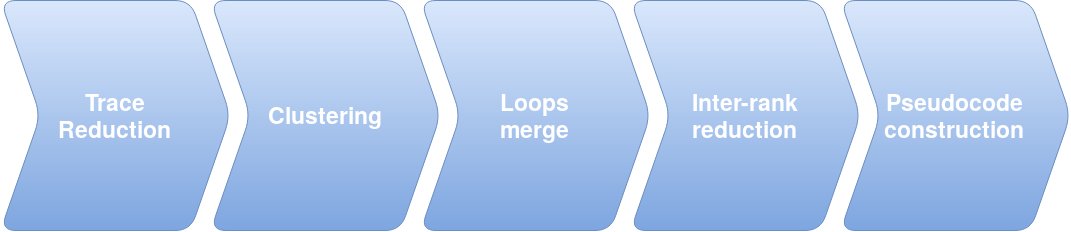
\includegraphics[width=\textwidth]{imgs/workflow.png}
	\caption{Structure detection workflow}
\end{figure}
\end{frame}

\begin{frame}
\frametitle{Workflow}
\framesubtitle{Trace reduction step (i)}
\textbf{Input} Tracefile, i.e. Sequence of timestamped events ordered by time.\\
\textbf{Output} Set of unique MPI calls with attached information.
\vspace{10px}
\pause
\begin{itemize}
	\item By \textbf{reduction} and \textbf{aggregation \& derivation}
	\item Is a sort of Map \& Reduce
	\item Every MPI call is identified by its \textbf{signature}
	\item Being the signature: Ordered sequence of pairs $(file,line)$ that define the call path, i.e. The dynamic position
\end{itemize}
\pause
\begin{figure}
	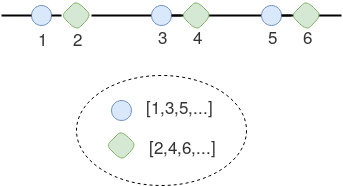
\includegraphics[width=0.5\textwidth]{imgs/workflow_reduction.png}
\end{figure}
\end{frame}

\begin{frame}
\frametitle{Workflow}
\framesubtitle{Trace reduction step (ii)}
Additionally \textbf{filter less representative MPI calls}.
\begin{itemize}
	\item Allows to decrease even more the clustering complexity.
	\item Focus only on the important data.
	\item The criteria is whether a given threshold of ``explained time'' is surpased.
\end{itemize}
\begin{equation}
	\delta(call) = \frac{it(call)*imt(call)}{T_{exe}}
\end{equation}
\begin{figure}
	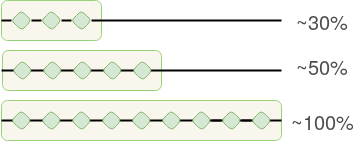
\includegraphics[width=0.5\textwidth]{imgs/workflow_reduction_2.png}
\end{figure}
\end{frame}

\begin{frame}
\frametitle{Workflow}
\framesubtitle{Trace reduction step (iii)}
The stored information for every unique MPI call is:
\begin{itemize}
	\item \textbf{Number of repetitions}
	\item \textbf{Mean time time between repetitions}
	\item Entire call path
	\item Previous burst performance information
	\item All timestamps
	\item Calculed delta
\end{itemize}
\vfill
\pause
\begin{block}{Keynote}
	HPC applications are strongly repetitive over time so number of unique MPI calls will remain despite the increasing problem size.
\end{block}
\end{frame}

\begin{frame}
\frametitle{Workflow}
\framesubtitle{Clustering}

\textbf{Input} Set of unique MPI calls with attached information.\\
\textbf{Output} Set of sets of MPI calls.
\vspace{10px}
\pause
\begin{itemize}
	\item \textbf{DBSCAN} as clustering algorithm (prefered to K-means)
	\begin{itemize}
		\item $\epsilon$ empirically set to 0.2 (in general)
		\item minPts set to 1
	\end{itemize}
\pause
	\item In a bidimentional space defined by
	\begin{itemize}
		\item Number of repetitions
		\item Mean time between repetitions
	\end{itemize}
\pause
	\item Resulting clusters \textbf{will be considered loops}.
	\begin{itemize}
		\item Since MPI calls acts as proxies
		\item Number of repetitions $\rightarrow$ Number of iterations.
		\item Mean time between repetitions $\rightarrow$ Mean iterations time.
	\end{itemize}
	
\end{itemize}
\end{frame}

\begin{frame}
\frametitle{Workflow}
\framesubtitle{Loops merge (i)}
\textbf{Input} Set of loops.\\
\textbf{Output} Set of top level loops with its related nested loops.\\
\vspace{10px}
\pause
Intuition
\begin{itemize}
	\item Isolated loops are just \textbf{pieces of the overall puzzle}.
	\item By discover its hierarchical relations \textbf{the structure of the application will be betrayed}.
\end{itemize}
\pause
Some clues
\begin{itemize}
	\item Outer loop will have \textbf{more iterations} then nested one.
	\item Outer loop will spend \textbf{more time} for per iteration.
	\item Outer loop will \textbf{explain the same amount of time} as inner loop.
\end{itemize}
\end{frame}

\begin{frame}
\frametitle{Workflow}
\framesubtitle{Loops merge (ii)}
\begin{multicols}{2}
	\begin{figure}
		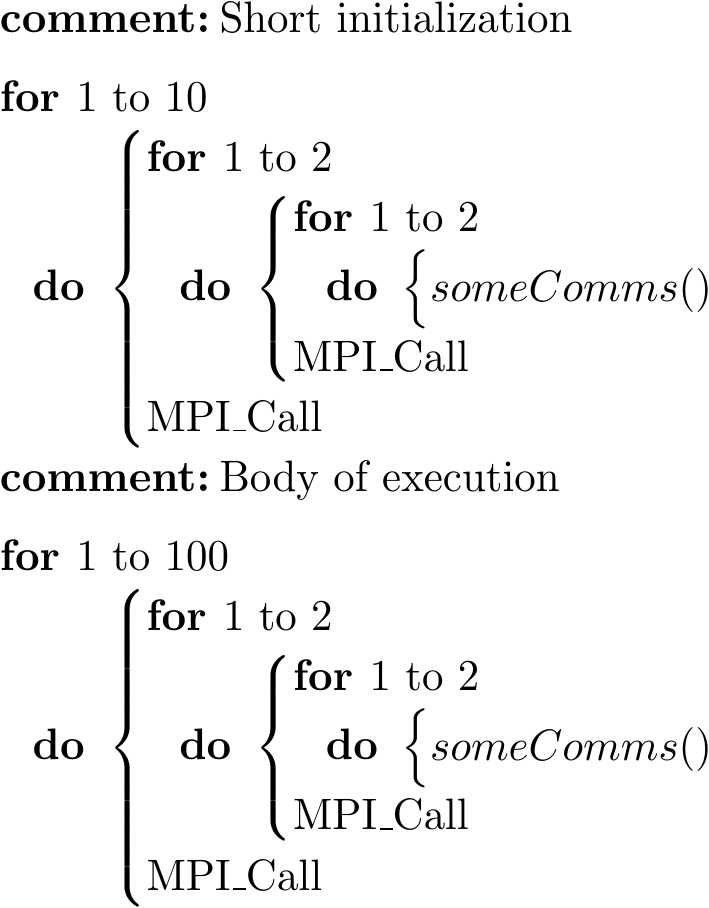
\includegraphics[width=0.3\textwidth]{imgs/delta_clustering_test_1_pse.png}
	\end{figure}
	\pause
	\columnbreak
	\begin{figure}
		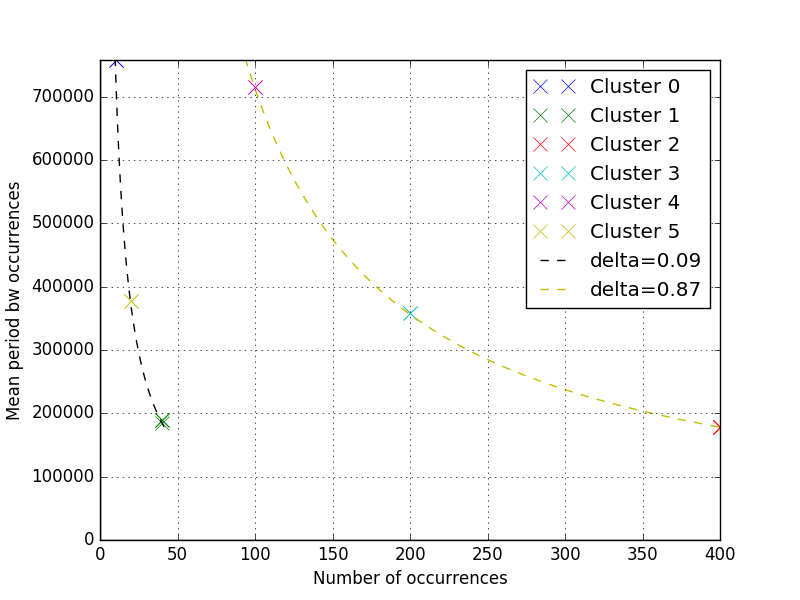
\includegraphics[width=0.5\textwidth]{imgs/delta_clustering_test_1.png}
	\end{figure}
\end{multicols}
\pause
\begin{block}{Keynote}
	Different phases can be detected by this way and used for the loops merging.
\end{block}
\end{frame}

\begin{frame}
\frametitle{Workflow}
\framesubtitle{Loops merge (iii)}
\begin{multicols}{2}
	\begin{figure}
		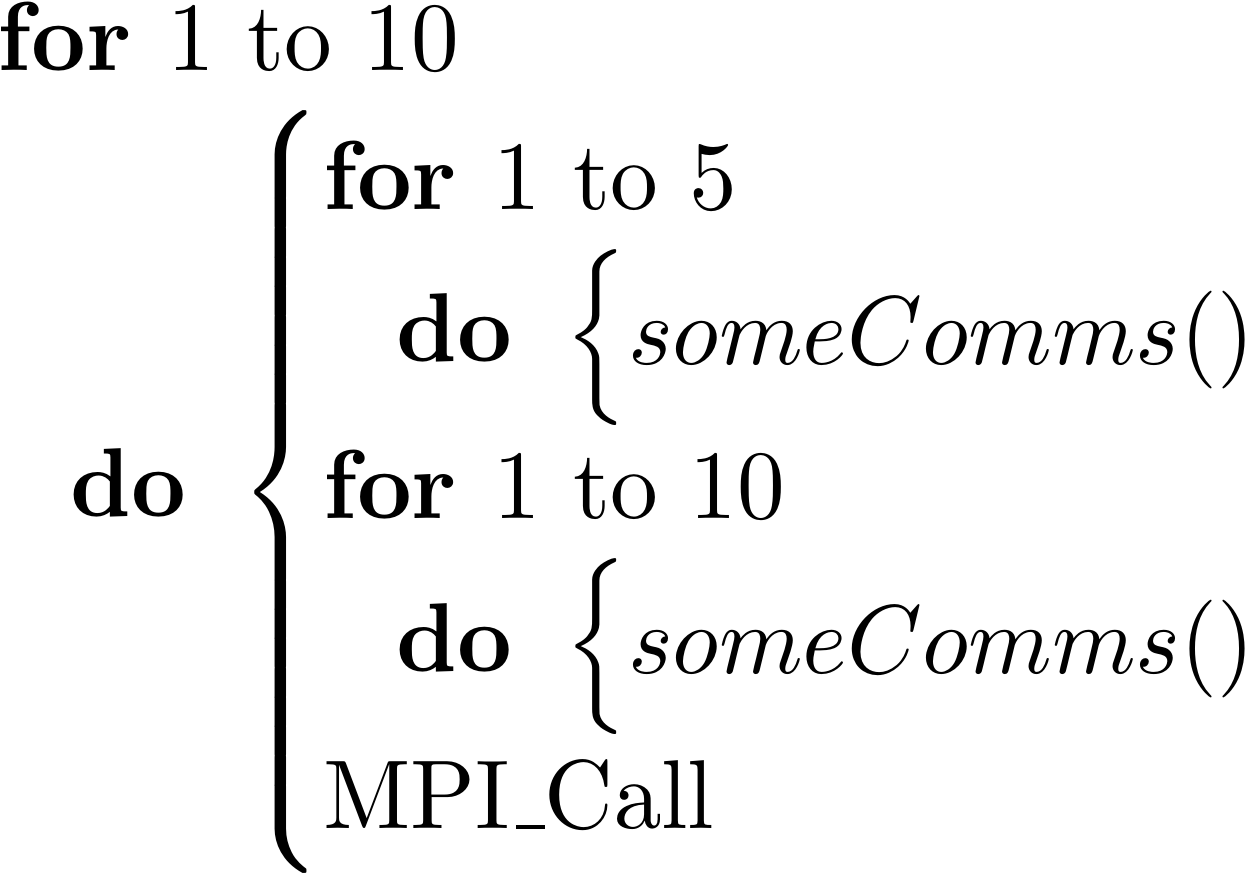
\includegraphics[width=0.4\textwidth]{imgs/delta_clustering_test_2_pse.png}
	\end{figure}
	\pause
	\columnbreak
	\begin{figure}
		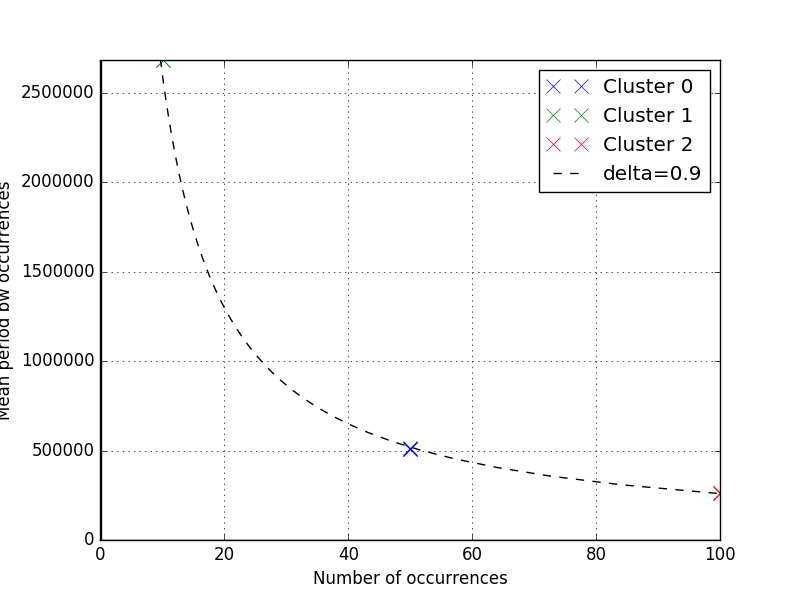
\includegraphics[width=0.5\textwidth]{imgs/delta_clustering_test_2.png}
	\end{figure}
\end{multicols}
\pause
\begin{block}{Warning}
	Not all loops that fulfills with nested loops conditions, are nested loops.\\
	Extra check is needed.
\end{block}
\end{frame}

\begin{frame}
\frametitle{Workflow}
\framesubtitle{Loops merge (iv)}
\begin{itemize}
	\item Classify MPI clusters/Loops ($\upsilon \in \Upsilon$) per ``how much of execution represents'' ($\delta \in \Delta$)\footnote{Do not confuse with $\delta()$ function.}.
	\item For every phase ($\delta$) sort loops ($\upsilon$) by number of iterations.
	\item Perform the loop merge \textbf{from high to low iterations count}.
	\item Before every merge, \textbf{check out} whether the hierarchical relationship is true.
\end{itemize}
\begin{figure}
	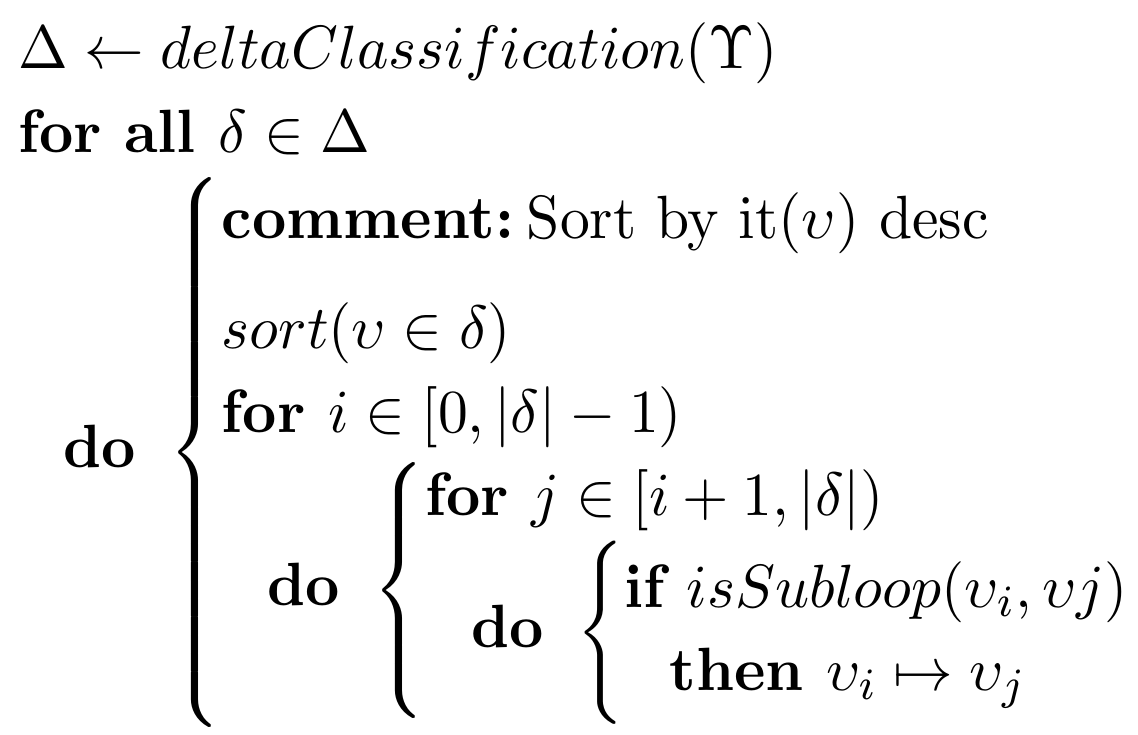
\includegraphics[width=0.5\textwidth]{imgs/loops_merge_pseudocode.png}
\end{figure}
\end{frame}

\begin{frame}
\frametitle{Workflow}
\framesubtitle{Inter-rank reduction (i)}
\textbf{Input} Set of top level loops.\\
\textbf{Output} Set of top level loops with rank conditional structures.\\
\vspace{10px}
\pause
\begin{itemize}
	\item Two calls with \textbf{same call paths still coexist} if belongs to different MPI ranks.
	\begin{itemize}
		\item \textbf{Conservative} reduction step! If assuming SPMD\footnote{Single Program Multiple Data} applications.
	\end{itemize}
	\item Divergences between MPI ranks are understood as \textbf{conditional structures in code}.
	\item This step is about: 
	\begin{enumerate}
		\item MPI Calls/Subloops ordenation
		\item Reduction
		\item Arrangement in conditional blocks
	\end{enumerate}

\end{itemize}
\end{frame}

\begin{frame}
\frametitle{Workflow}
\framesubtitle{Inter-rank reduction (ii)}
\begin{multicols}{3}
	\vfill
	\begin{figure}
		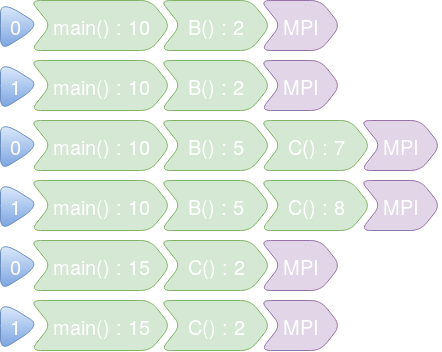
\includegraphics[width=0.3\textwidth]{imgs/workflow_ranks_1.png}
		\caption{Ordenation}
	\end{figure}
	\columnbreak
	\pause
	\begin{figure}
		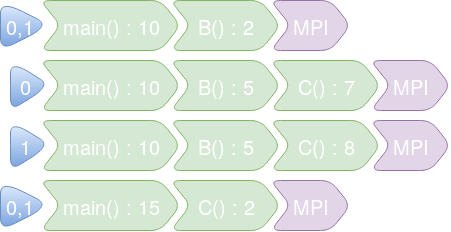
\includegraphics[width=0.3\textwidth]{imgs/workflow_ranks_2.png}
		\caption{Reduction}
	\end{figure}
	\columnbreak
	\pause
	\begin{figure}
		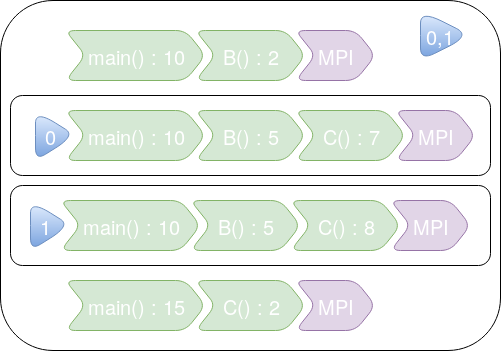
\includegraphics[width=0.3\textwidth]{imgs/workflow_ranks_3.png}
		\caption{Conditional blocks}
	\end{figure}
\end{multicols}
\end{frame}

\begin{frame}
\frametitle{Workflow}
\framesubtitle{Pseudocode construction (i)}
\textbf{Input} Set of top level loops with rank conditional structures.\\
\textbf{Output} Pseudocode representing the actual application structure. \\
\vspace{5px}
\pause
\begin{itemize}
	\item Straightforward construction
	\item For bettern understanding \textbf{repetitive information from call paths is removed}.
	\begin{enumerate}
		\item Extracting common call path levels from code block (loops and conditional blocks)
		\item Removing \textbf{contiguous repetitive information} what has not been removed in previous step
	\end{enumerate}
\end{itemize}
\begin{multicols}{3}
	\begin{figure}
		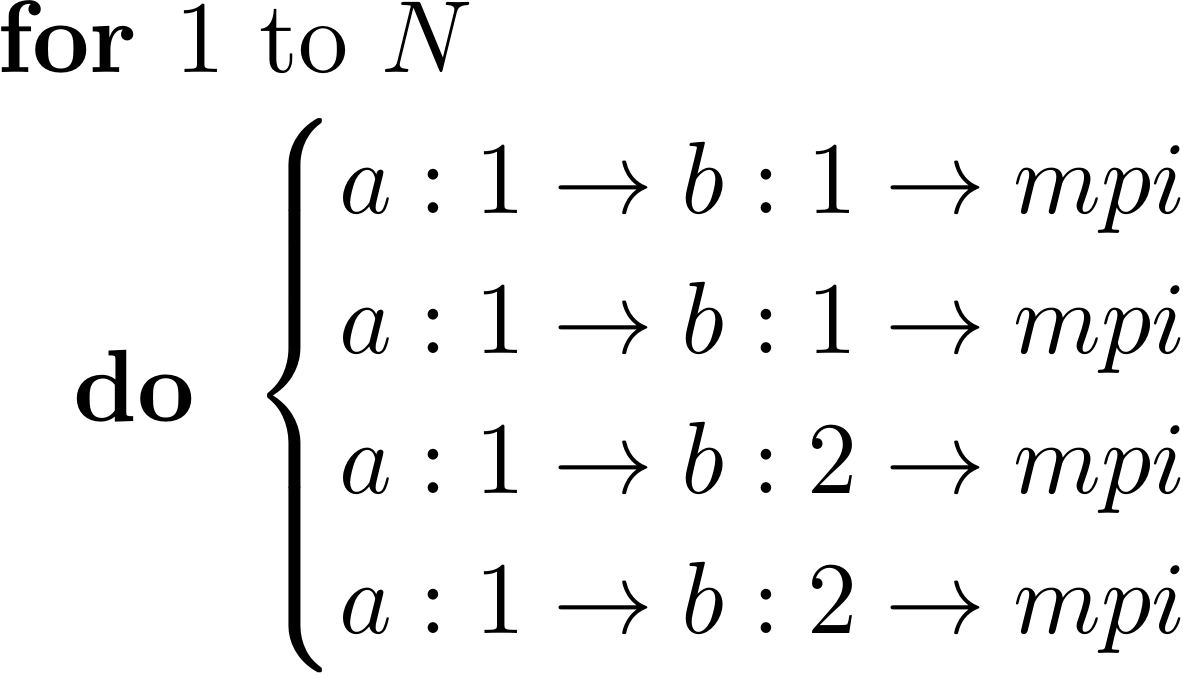
\includegraphics[width=0.3\textwidth]{imgs/workflow_pseudocode_1.png}
		\caption{Raw pseudocode}
	\end{figure}
	\columnbreak
	\pause
	\begin{figure}
		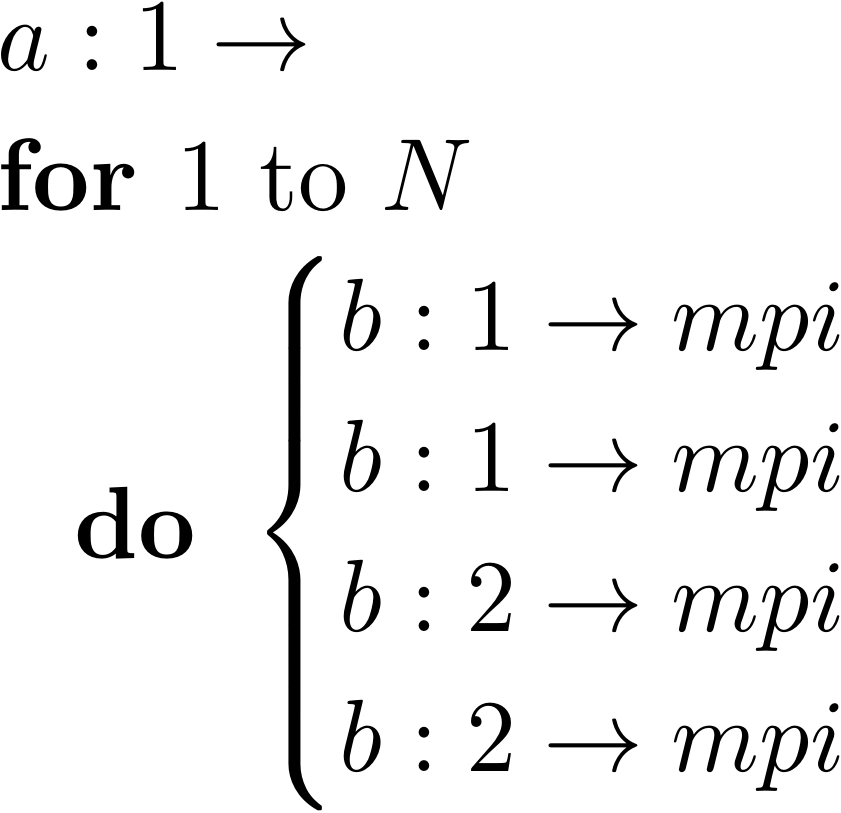
\includegraphics[width=0.18\textwidth]{imgs/workflow_pseudocode_2.png}
		\caption{After extract common call path}	
	\end{figure}
	\columnbreak
	\pause
	\begin{figure}
		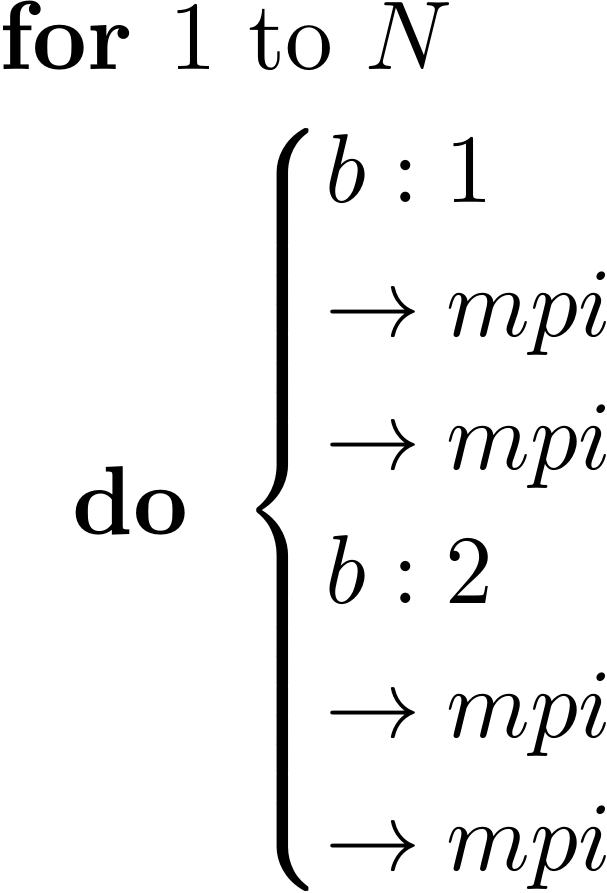
\includegraphics[width=0.14\textwidth]{imgs/workflow_pseudocode_3.png}
		\caption{After extract contiguous call path}
	\end{figure}
	\columnbreak
\end{multicols}
\end{frame}

\begin{frame}
\frametitle{Workflow}
\framesubtitle{Pseudocode construction (ii)}
\begin{figure}
	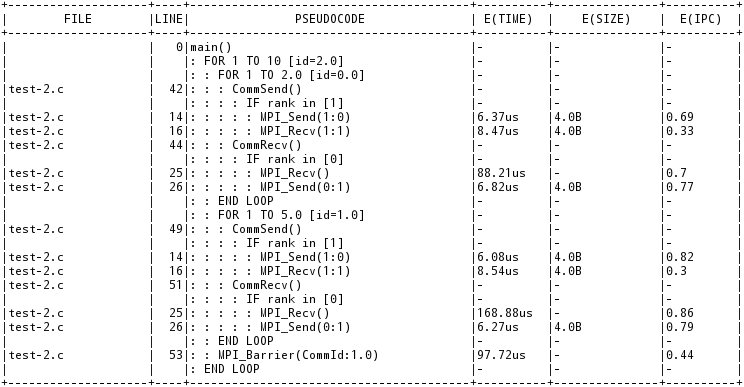
\includegraphics[width=0.7\textwidth]{imgs/console_gui_example_1.png}
	\caption{Example console output}
\end{figure}
\pause
\begin{itemize}
	\item Additionally an \textbf{interactive shell} is provided to the user allowing...
	\begin{enumerate}
		\item Show cpu burst metrics over a given thresshold.
		\item Filter by MPI rank.
		\item Show clustering plot.
		\item ...
	\end{enumerate}
\end{itemize}
\end{frame}

\section{Further considerations}
\begin{frame}
\frametitle{Further considerations}

Until now were not aware \textbf{the problems can arise from clustering step}. \\
But there are some:
\begin{enumerate}
	\item \textbf{Cluster aliasing} when two different loops behaves similarly enough over our defined space
	\item \textbf{Cluster split} when MPI calls belonging to the same loop behaves in a different way.
\end{enumerate}
\vfill
\pause
\begin{multicols}{2}
	\begin{figure}
		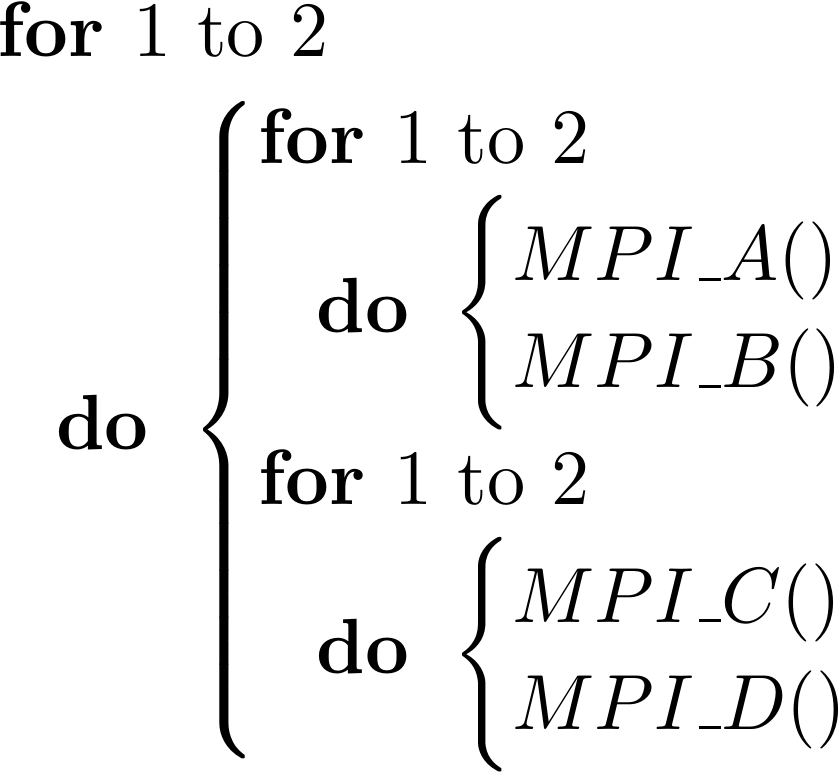
\includegraphics[height=80px]{imgs/aliasing_example.png}
		\caption{Cluster aliasing example}
	\end{figure}
	\columnbreak
	\begin{figure}
		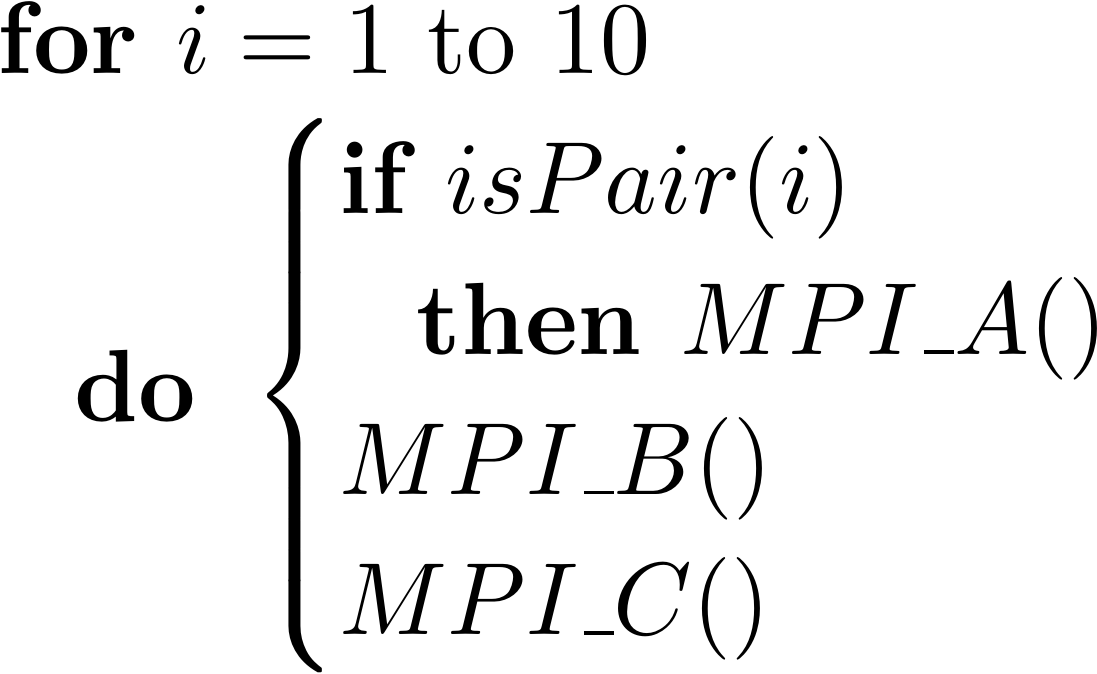
\includegraphics[height=80px]{imgs/split_example.png}
		\caption{Cluster split example}
	\end{figure}
\end{multicols}
\end{frame}

\subsection{Data analysis}

\subsection{Proposal modifiations}

\section{Results}
\subsection{Specific capabilities}
\begin{frame}
Hola manola
\end{frame}
\subsection{Real application}
\begin{frame}
Hola manola
\end{frame}

\section{Conclusions}
\begin{frame}
Hola manola
\end{frame}

\bibliography{bibliography}
\bibliographystyle{apalike}

\end{document}